\section{Introduction}\label{sec:Intro}
Galaxies are complex structures consisting of stars, gas, dust and \ac{DM} held together by gravity. They have many different shapes, colors and sizes, from low mass \ac{DG} to very massive elliptical galaxies, and are in constant change induced by stellar evolution and, with greater impact, by galaxy mergers. We can observe galaxies over a range of scales: from our Galaxy, the \ac{MW}, over nearby galaxies, where we can still resolve individual parts, to high-redshift galaxies, when the Universe was still very young. This range of galaxies gives insight on galaxy formation and evolution through cosmic times. In their similarities, we can constrain many physical laws about galaxies and the Universe. 

\subsection{The importance of knowing the gravitational potential of galaxies}
One of the most fundamental galaxy properties is its mass. As astronomers, we are interested in the total mass, and also how that mass is distributed, as the mass distribution gives rise to a gravitational potential that governs how the objects in the potential move. Many empirical correlations for galaxies were found which rely on the velocity dispersion, therefore mass, therefore potential of a galaxy. \\
Galaxies are made up of visible matter (stars, gas, dust) and invisible matter (\ac{DM}). Through observations of the visible components, we can make educated estimates of their mass, but we cannot measure the mass of \ac{DM} directly as we cannot see it. However, \ac{DM} dominates the mass budget of galaxies, so it is very important for our understanding how mass is distributed in galaxies, and throughout the Universe.

\subsubsection{Dark matter}
\ac{DM} is invisible in all parts of the electromagnetic spectrum, so it can only be observed indirectly via the gravitational effect it has on objects that we can see. We will now give a very quick overview on the discovery, most promising models, problems and alternatives. This Section closely follows the review chapter on \ac{DM} in Wilma Trick's PhD thesis \citep{Wilmathesis}; the main references are \citet{Ostriker...DM...2003, Maoz...astrophysics...2007} and \citet{Mo...galformev...2010}. \\
\\\textbf{History of \ac{DM} discovery} In 1933, \citeauthor{Zwicky...DM...1933} observed the motions of galaxies in the Coma clusters and found a much higher velocity dispersion than expected from the visible matter after applying the virial theorem. He introduced the term "dunkle Materie" (German for dark matter) which described the invisible matter. Almost 40 years later, Rubin \textit{et al.} \citeyearpar{Rubin...DM...1970, Rubin...DM...1978, Rubin...DM...1980} measured rotation curves of first the Andromeda galaxy, our closest spiral galaxy, then of many other edge-on disk galaxies. The visible mass content would lead to rotation curves that decreased towards higher radii $r$ but the rotation curves stayed constant over a large radial range following 
\begin{equation}\label{eq:circ_vel}
    v_{\mathrm{circ}}(r) = \sqrt{\frac{GM(r)}{r}} \sim \mathrm{constant}
\end{equation}
with the circular velocity $v_\mathrm{{circ}}(r)$, the gravitational constant $G$ and the total mass within the radius $M(r)$, indicating that there are halos around galaxies built up from invisible matter. Other observational methods also rely on \ac{DM}, such as strong (e.g. \citealp{Trick..stronglensing...2016}) and weak gravitational lensing \citep{Tyson...weaklensing...1990, Kaiser...weaklensing...1993}. \ac{DM} seems to only interact via gravitational forces but not with electromagnetic radiation and therefore cannot be observed by light. Unfortunately, up to now, there has not been a direct detection of \ac{DM} in any way which causes great challenges but also brings many opportunities of research.\\
\\\textbf{Cosmological aspects of \ac{DM}}
In the current standard model of cosmology, the \ac{LCDM}-model, the Universe is made up of dark energy ($\Lambda$) and matter. Recent measurements of the cosmic microwave background by the \citet{Planck...CMB...2018} found that dark energy makes up the biggest fraction of the energy density ($\Omega_\Lambda = 0.685$) and matter the rest ($\Omega_m = 0.315$), split up to $\Omega_b = 0.05$ baryonic matter and $\Omega_c = 0.265$ cold dark matter assuming a Hubble constant of H$_0$ =  \SI{67.27}{km.s^{-1}.Mpc^{-1}}. Therefore, \ac{DM} makes up around \SI{84}{\%} of the total matter in the Universe. \\
\\\textbf{Established \ac{DM} model - cold dark matter}
Cold dark matter (\acsu{CDM}) was first introduced by \cite{Davis....CDM...1985} through \textit{N}-body simulations. \ac{CDM} particles are long-lived and very massive (\SI{10}{GeV} to a few TeV). These particles decoupled very early in the beginning stages of the Universe, already before reionization, and therefore are nonrelativistic. The particles were scattered almost homogeneously throughout the Universe, but with some very small fluctuations. In slightly overdense regions there was a slightly stronger gravitational pull, and in underdense regions slightly less, so particles moved towards the overdense regions and away from the underdense regions. Over time, the particles clustered, forming increasingly larger structures: this bottom-up picture of structure formation is known as hierarchical growth. Baryonic matter moves towards the overdense regions as well and galaxies form in the deepest \ac{DM} potential wells and along the \ac{DM} filaments (Figure \ref{fig:DM_stars_AU24} shows this structure in the simulation we introduce in Section \ref{sec:Auriga}). Relativistic particles would destroy small scale substructure which would lead to larger voids than we observe. Possible particle candidates are Weakly Interacting Massive Particles which are massive particles interacting only via gravity and the weak force. The large scale structure predicted by \ac{CDM} simulations agrees extraordinary well with the observed clustering of galaxies (e.g. in the Millenium simulations, \citealp{Springel...Millenium...2005}). \\
\\\textbf{Problems in the current model}
Although successful in explaining many large-scale phenomena, \ac{CDM} has some problems on especially smaller scales (< \SI{1}{Mpc}) when comparing the predictions of cosmological \ac{DMO} simulations to observations (e.g., see the review by \citealp{Bullock...LCDMprobs...2017}). Some of these problems have been remedied in the recent years.
\begin{itemize}
    \item\textbf{The missing satellites problem:} These simulations predict many more satellites of galaxies in the low-mass end than we observe \citep{Klypin...missingsatellites...1999, Moore...missingsatellites..1999}. This can be explained by the fact that low mass \ac{DM} halos are extremely ineffective in forming galaxies and go completely dark below a certain threshold mass. In recent simulations analyzed by \citet{Sawala...noCDMproblems...2016} including baryons and physical prescriptions, the number of satellites matched the observations.
    \item \textbf{The cusp-core problem:} In these \ac{DMO} simulations, the halo density profile has a cusp in the center (e.g. \citealp{Dunbinski...DMCusp...1991, Navarro...DMCusp...1996}) while observations find flatter density profiles and cored centers \citep{Flores...cuspcoreprob...1994, Moore...cuspcoreprob...1994}. Simulations that include baryons have shown that baryonic feedback processes can flatten cusps into cores (e.g. \citealp{Pontzen...cuspcore..2012}). 
    \item \textbf{The too-big-to-fail problem} \citep{Boylan...toobigtoofail...2011}\textbf{:} In the \ac{DMO} simulations, a large population of \ac{DM} satellites are found with greater central masses than any of the \ac{MW}'s dwarf spheroidals. These subhalos seem to have failed to form galaxies while halos with lower mass were successful. It was first found for the \ac{MW} but the same problem occurs for Andromeda \citep{Tollerud...M31tbtf...2014}, other Local Group galaxies \citep{Kirby...LGtbtf...2014} and in more isolated lower mass galaxies \citep{Ferrero...DGtbtf...2012, Papastergis...DGtbtf...2015, Papastergis...DGtbtf...2016}.
    \iffalse\item The planes of satellites problem: \fi
\end{itemize}

\textbf{\ac{CDM} alternatives} Many alternatives for \ac{CDM} have been suggested and many of them have already been ruled out. Some of the alternatives which still are considered are 
\begin{itemize}
    \item \textbf{Warm dark matter} These particles should have masses of around \SI{1}{keV}. The mass grows hierarchically down to a characteristic mass scale, below which the free streaming of the particles prevents halos from forming and the \ac{DM} is distributed in a smooth background field instead \citep{Smith...WDM..2011, Schneider...WDM...2013}. This theory predicts fewer low-mass \ac{DM} halos whose densities would be less cuspy in the centers due to higher thermal motions \citep{Bode...WDM...2001}.
    \item \textbf{\ac{MoND}:} \cite{Milgrom...MoND...1983} suggested the idea of a modified theory of Newtonian law of gravity which only has an effect in low accelerations. This theory explains flat rotation curves. A big advantage would be the non necessity of a new mysterious dark particle. Nevertheless, there are examples such as the Bullet cluster \citep{Clowe...Bullett...2006} which fit perfectly in the \ac{CDM} universe but struggle to find an explanation in \ac{MoND}.
\end{itemize}

\subsubsection{Empirical galaxy correlations}
In galaxies, many characteristics appear to be correlated. These correlations are usually found empirically by analyzing and combining observational results. Many of the correlations include the mass of a galaxy so once we know the mass we can also make inferences about other properties of the galaxy. 
\begin{itemize}
    \item \textbf{\citet{Tully...Fisher...1977}} (TF) determined a relationship between the luminosity L of a spiral galaxy and its radial velocity (which is connected to the mass of a galaxy through Equation \ref{eq:circ_vel}):
    \begin{equation}
        L \propto (v_{\mathrm{circ, max}})^\beta \qquad \mathrm{with}\quad \beta =  2.5 - 5
    \end{equation}
    For the radial velocity, they measured the Doppler-broadened 21-cm radio emission line of neutral hydrogen (see Section \ref{subsec:mass_est_ext}). 
    \item \textbf{\citet{Faber...Jackson...1976}} measured the central radial velocity dispersion $\sigma_0$ of elliptical galaxies and found the relation to the luminosity  
    \begin{equation}
        L \propto \sigma_0^4,
    \end{equation}
    which is similar to the \acs{TF} relation of spiral galaxies. The derivation of this relation made simple assumptions such as a uniform mass distribution on the volume of radius \textit{R} and a constant mass-to-light ratio for all galaxies and equal surface brightnesses. These assumptions are not entirely correct, so there is a large scatter in the data around this relation.
    \item \textbf{The Fundamental Plane} offers a better empirical fit to the data of elliptical galaxies but needs another parameter, the effective radius $r_e$. It combines radius and luminosity of a galaxy with its gravitational well. Two representations of the fit are \citep{Carroll...Ostlie..2006}:
    \begin{align}
        L &\propto \sigma_0^{2.65}r_\mathrm{e}^{0.65} \\
        r_\mathrm{e} &\propto \sigma_0^{1.24}I_\mathrm{e}^{-0.82}.
    \end{align}
    Dynamically hot stellar systems, i.e. stellar systems whose stars are on randomized orbits, follow this scaling relation \citep{Misgeld...hotss.FP...2011}.
    \iffalse\item M\_vir - N\_GC \fi
\end{itemize}

\iffalse
\subsubsection{Application}
MW \acp{GC} proper motions and dynamics (including action distribution and dynamical model of potentials): \cite{Vasiliev...GCoverview...2018}\\
Modelling the \ac{MW}'s \ac{GC} system: \cite{Binney...GCsystem...2017}
\fi
\subsection{Dynamical modelling methods}
As we are not able to observe \ac{DM} directly, we cannot measure the mass and position of each \ac{DM} particle. Indeed, our ability to do this for visible matter is limited even in the \ac{MW}, and impossible in more distant galaxies. Instead, we measure velocities of visible objects that move under the influence of the mass distribution. To connect these velocity measurements to the underlying physics, and hence to infer a gravitational potential, we use dynamical models. Stars in the disk and in the halo of galaxies can be considered as collisionless tracers so the \ac{CBE} (Equation \ref{eq:CBE})  applies to them.
\begin{itemize}
    \item \textbf{Jeans modelling} \citep{Jeans.....1915}: The first velocity moment of the \ac{CBE} relates the velocity ellipsoid of stars at a given position in a galaxy to the gravitational forces and the spatial \ac{DF} - for an explanation of \acp{DF} see Section \ref{subsubsec:pot_theory} - of the stars. One important advantage of this method is that the computation is fast so a lot of different models can be explored. One disadvantage is that the set of Jeans equations is not closed and therefore does not have a unique solution. Therefore, assumptions need to be made and the solution, if found, may give non-physical results e.g. a negative \ac{DF} (e.g. \citealp{Eilers...Jeans...2018}). 
    \item \textbf{Schwarzschild's orbital superposition approach} \citep{Schwarzschild...1979}: Dynamical models of triaxial galaxies can be made based on observed surface brightness distribution and observed kinematics. Given a potential, an orbit library over the full integral of motion space is constructed. The number/mass/light of stars on a specific orbit are described by a weight. These weighted orbits build up the stellar \ac{DF}. By comparing the surface brightness and kinematics of the model with the data, the gravitational potential can be recovered. This method is mostly used in external galaxies \citep{Rix...Schwarzschild...1997, vdBosch...Schwarzschild...2008, Vasiliev...Schwarzschild...2013, Ling...Schwarzschild...2018}.
    \item \textbf{Action-based modelling:} Orbits in axisymmetric potentials can be modelled with \acp{DF} which arrange stars in 3D action space instead of 6D phase-space \citep{Binney...actionbasedmodelling...2012, Bovy...actionbasedmodelling...2013}. The modelling is similar to the Schwarzschild approach. The differences are that it does not numerically integrate orbits but uses orbital actions and tori and instead of orbits weights, the analytic \acp{DF} are physically motivated and action-based. Since we need 6D phase-space information to calculate actions it is mainly used in the \ac{MW} where we can resolve single stars. It is applied to modelling the disk (e.g., \citealp{trick...ROADMAPPING...2016, Wilmathesis}) but also to model the stellar halo (see Section \ref{subsec:mass_est_MW}). 
\end{itemize}
\subsection{Some stellar objects in the halos of galaxies}\label{subsec:halo_objects}
\textbf{Globular clusters\acused{GC} (\acp{GC})} are self-gravitating, gravitationally bound, gas and \ac{DM}-free systems of $10^5$ to $10^7$ stars which are spherically grouped with a typical size of a few parsecs and mass around $10^5$ to $10^6\ \mathrm{M}_\odot$. They are therefore much brighter than stars but still very compact so they can be resolved in external galaxies. Since they are some of the oldest stellar populations in the Universe (approximately \SI{13}{Gyr} old), the chemical composition and kinematics of the \ac{GC} population contain much information about the assembly history and evolution of the \ac{MW} and external galaxies. The \ac{MW} is known to host two distinct \ac{GC} populations: metal-poor vs. metal-rich / blue vs. red / no net rotation vs. corotation / in halo vs. centrally concentrated / probably accreted vs. in-situ (\citealp{Renaud...MWGCs....2017} and references therein). \\\\
\textbf{Stellar streams} are remnants of tidally disrupted \acp{GC} or \acp{DG} and are a byproduct of hierarchical galaxy formation. A dynamically cold stream - which means it has a low intrinsic velocity dispersion - usually originates from a \ac{GC} \citep{Bonaca...streamsinfo...2018}. Their phase-space distribution is predominantly affected by the galactic gravitational potential and depends less on internal kinematics \citep{Kupper...streams...2010, Kupper...streams...2012}. They are very thin and more than twice as long as wide so they can be treated as one dimensional in the plane of the sky \citep{Bonaca...streamsinfo...2018}. Hot stellar streams are created by satellites with higher velocity dispersions such as \acp{DG}. The first detected and since then often investigated (hot) stellar stream is the Sagittarius dwarf galaxy and its tidal arms \citep{Ibata...Sagittarius....1994}.\\
%\textbf{\textcolor{red}{The diffuse stellar halo}}\\
%\textbf{\textcolor{red}{DG satellites around large galaxies (mass,size,dm,AMR)}}
\subsection{Strategies to model the Milky Way potential}\label{subsec:mass_est_MW}
There are many different approaches for measuring the mass and the potential of the Galaxy. Due to our position within the \ac{MW}, some methods which give very good constraints on overall parameters such as e.g. rotation curves of external galaxies (see Section \ref{subsec:mass_est_ext}) cannot be measured as easily. A big advantage is that we can resolve stellar positions and velocities with high precision, especially with \textit{Gaia} \citep{Gaia...mission...2016, GaiaDR2...overview...2018, GaiaDR...GCs...2018}, which is helpful in both Galactic archaeology and dynamical modelling. These are some of the kinematic and dynamical methods to measure the Galactic mass in the halo (their results are presented in Table \ref{tab:MW_mass_estimations}):
\begin{itemize}
    \iffalse\item Kinematics of nearby stars: \cite{Kuijken...LocalDMdens...1989, Bovy...LocalDMdens...2012} \fi
    \item \textbf{Orbits of stellar streams:} \citet{Johnston...MWstreams...1999} first found that stellar streams contain information about the Galaxy's gravitational potential. In the case of kinematically cold streams, they move on orbits aligned with the remnant's orbit \citep{Eyre...streamstheo...2011}. It is therefore possible to get a direct measurement of the local acceleration close to the stream. So far, dynamical models of four single stellar streams have been used to constrain the mass and shape of the \ac{DM} halo: the Sagittarius dwarf galaxy \citep{Law...sagstream...2010, Gibbons...sagstream...2014, Dierickx...sagstream..2017}, the Orphan stream \citep{Newberg...orphanstream..2010}, the GD-1 stream \citep{Koposov...GD1stream...2010, Bowden...GD1stream...2015, Malhan...GD1stream...2018}, and the tails of the Palomar 5 globular cluster \citep{Kupper...pal5stream...2015}. Since these streams measure local properties, better constraints on the global potential can be achieved by looking at a population of streams \citep{Bonaca...streamsinfo...2018}.
    
    \item \textbf{Stellar streams in action space:} The phase-space distribution of tidal streams have the simplest form in action-angle-frequency space \citep{Tremaine...streamsactiontheory...1999, Helmi...streamsactionstheory...1999}. A deeper introduction to actions is given in Section \ref{sec:Dynamics}. Due to formerly-high computing costs for calculating actions numerically, this approach has been carried out on larger scales only recently after developing new, cheaper methods for action calculations (a review is given in \citealp{Sanders...actionreview...2016}). \citet{Streams...Sanders...2014} uses a St\"ackel-fitting algorithm \citep{Sanders...Staeckel...2012} to generate probabilistic models of streams to constrain the Galactic potential. \citet{Streams...Bovy...2014} introduces a new, general method of action-angle-frequency calculation for streams using an orbit-integration-based approximation. In \citet{Streams..GD1..Pal5...Bovy...2016}, this method is then for the first time applied individually and combined to the Palomar 5 and GD-1 streams.
    \item \textbf{Tracer dynamics:} Another tracer of the mass of the inner \ac{MW} halo ($r\le$ \SI{21}{kpc}) is the \ac{GC} distribution. There have been a lot of previous studies on this method (for a review see \citealp{Bland-Hawthorn...MW...2016}) but the best constraints come from recent advances that give us full 6D phase-space information. As part of the second \textit{Gaia} data release, \citet{GaiaDR...GCs...2018} calculated \acp{PM} for 75 \acp{GC}; \citet{Vasiliev...GCoverview...2018} and \citet{Baumgardt...GCoverview...2019} later expanded the sample, calculating \acp{PM} for 150 and 154 \acp{GC} respectively. \citet{MWmass...GCmotions...Watkins...2018} use the kinematics of a subsample of \acp{GC} in this inner halo to constrain the Galaxy's mass using a simple tracer mass estimator. \citet{Posti...MWmassGCs...2019} employ another approach based on \citet{Binney...MWGCModel....2017} by fitting an action-based \ac{DF} to the 6D phase-space data of 75 \acp{GC} to constrain the mass and shape of the \ac{DM} halo. A very similar approach is carried out in \citet{Vasiliev...GCoverview...2018} which mainly differs in assumptions on the assumed form of the halo. \acp{PM} are measured by other telescopes as well. \citet{Sohn...GCsHST..2018} use Hubble Space Telescope \acp{PM} to derive the mass of the \ac{MW} with the same method as \citet{MWmass...GCmotions...Watkins...2018} but fewer \acp{GC}. \citet{Eadie...GCsBayes...2018} apply a hierarchical Bayesian model to the samples from \citet{Vasiliev...GCoverview...2018} and \citet{Sohn...GCsHST..2018}.
    \\ To constrain the mass of the outer halo we can use satellite galaxies as tracers. The methods are similar to the ones used for \ac{GC} estimates. From position and velocity of the most distant dwarf Leo I ( $r= 257.8_{{-35.1}}^{+16.8} $ kpc), \citet{GaiaDR...GCs...2018} provided a lower limit on the \ac{MW} mass. \citet{MWmass...sat...dyn} calculate in the hydrodynamical simulations \acp{DF} of specific energy and angular momentum, with given 6D phase-space information, which vary according to the galaxy host mass, estimate this mass by a maximum likelihood and apply this method to the \ac{MW}.
\end{itemize}

\begin{table}[htbp]
\captionsetup{format=plain}
    \centering
    \caption{Mass estimation results of the \ac{MW} for some of the mentioned references. Empty values were not indicated in the papers.}
    \begin{tabular}{@{}lrrrrl@{}}
         \toprule
         \makecell[tl]{Method}& \makecell[tr]{$M_\mathrm{MW}$\\\newline[$10^{11} \mathrm{M}_\odot$]} & \makecell[tr]{at $R$ \\\newline[kpc]}&\makecell[tr]{$v_\mathrm{circ}$ \\\newline[km s$^{-1}$]\\at $R_\odot$}&$q$ & \makecell[tl]{Reference}  \\
         \midrule
         Stellar & $4.1 \pm 0.4$& 100 &&&\citetalias{Gibbons...sagstream...2014} \\
         streams& $<10$&&&&\citetalias{Dierickx...sagstream..2017}\\
         &$2.6$&$60$&&&\citetalias{Newberg...orphanstream..2010}\\ 
         &&&$224_{{-14}}^{+12}$&$0.87_{{-0.04}}^{+0.07}$&\citetalias{Koposov...GD1stream...2010}\\
         &&&$227.3_{{-18.2}}^{+15.6}$&$0.9_{{-0.1}}^{+0.04}$&\citetalias{Bowden...GD1stream...2015}\\
         &$1.75_{{-0.05}}^{+0.06}$&$14.5$&$244.4_{{-2}}^{+6}$&$0.86_{{-0.07}}^{+0.04}$&\citetalias{Malhan...GD1stream...2018}\\
         &$2.1\pm0.4$&$19$&$253\pm16$&$0.95_{{-0.12}}^{+0.16}$&\citetalias{Kupper...pal5stream...2015}\vspace{3mm}\\
         &$1.1\pm0.1$&$20$&&$0.94\pm0.05$&\citetalias{Streams..GD1..Pal5...Bovy...2016}\vspace{3mm}\\
         Tracer&$2.2_{{-0.03}}^{+0.04}$&21.1&&&\citetalias{MWmass...GCmotions...Watkins...2018}\\
         dynamics&$1.91_{{-0.17}}^{+0.18}$&$20$&&&\citetalias{Posti...MWmassGCs...2019}\\
         &$6_{{-0.09}}^{+0.14}$&$50$&&&\citetalias{Vasiliev...GCoverview...2018}\\
         &$6.1_{{-0.12}}^{+0.18}$&$39.5$&&&\citetalias{Sohn...GCsHST..2018}\vspace{3mm}\\
         & $3.3_{{-0.7}}^{+1.1}$&$39.5$&&&\citetalias{Eadie...GCsBayes...2018}\vspace{3mm}\\
         &$9.1_{{-2.6}}^{+6.2}$&$257.8_{{-35.1}}^{+16.8}$&&&\citetalias{GaiaDR...GCs...2018}\\
         &$10.4_{{-0.14}}^{+0.23}$&\makecell[tr]{$R_{200}$\\not specified}&&&\citetalias{MWmass...sat...dyn}\\
         \bottomrule 
    \end{tabular}
    \label{tab:MW_mass_estimations}
\end{table}
An overview of the results is shown in Table \ref{tab:MW_mass_estimations}. We see, that different methods allow us to constrain the potential at different distances, to the outermost tracers. However, this makes it more complicated to compare the results as masses need to be extrapolated to estimate the total mass. The estimates where q is given use a logarithmic halo potential for the \ac{DM} halo given by $\Phi(R,z) = v_\mathrm{circ}^2/2\ \mathrm{ln}(R^2 +z^2/q^2 + \mathrm{core}^2)$ where the core is the radius at which the logarithm is cut and $q$ is the $z$-flattening parameter which defines the ellipticity (oblate or prolate) of the \ac{DM} halo (see e.g. \citealp{Malhan...GD1stream...2018}).  

\subsection{Strategies to measure the mass of external galaxies}\label{subsec:mass_est_ext}
In external galaxies, we cannot resolve single stars; in some cases, depending on mass, luminosity and distance of the galaxy, we can resolve objects in the halo such as \acp{GC}, in other cases, we can only observe a galaxy as point source on the sky. To get a constraint on their mass it is useful to measure the rotational velocity of the galaxy (see Equation \ref{eq:circ_vel}). Different techniques evolved over time and telescope resolution, from measuring one value of the velocity to having spectra for each observed pixel. Some of them are:
\begin{itemize}
    \item\textbf{1D: 21cm line} Hydrogen is the simplest yet most abundant atom in space. The 21 cm line of neutral hydrogen (HI line) is visible through photons which are emitted when relative spins change from parallel to antiparallel. HI is detectable in radio bands in most spirals and some ellipticals. Line-of-sight velocities can be measured from the Doppler shift of these emission lines which give us a constraint on the galaxy's disk maximum rotation velocity and therefore a measurement of the enclosed mass.
    \item\textbf{2D: slit along the major axis} With the slit of a spectrograph aligned along the major axis of a galaxy, it is possible to take stellar spectra at different galactocentric radii. These spectra give us for a population of stars the line-of-sight velocity and the velocity dispersion which both are useful in dynamical modelling. Stars moving towards the observer are blue-shifted, stars moving away are redshifted. From the Doppler shift one can derive the rotational velocity and therefore the mass. 
    \item \textbf{3D: \acl{IFU}} \ac{IFU} spectrographs observe the 2D field of view and take a spectrum for each pixel at the same time. With that method we gain a 2D velocity map and can learn more about the mass distribution of the observed galaxy. From the spectra of \acp{GC} we can extract information with spectral synthesis on age, mass, metallicity and other important characteristics. 
    \iffalse\item \textbf{\textcolor{red}{point sources in the halo (GCs, PNe, satellite DGs, ...)}}\fi
\end{itemize}

\subsection{Idea of this thesis: Adaptive dynamics of accreted globular clusters}
\textbf{Context}
As we have seen, there are several methods of measuring the mass of external galaxies which rely mainly on the rotational velocities measured for unresolved stellar populations. We can try to adapt some of the methods which we use in the \ac{MW} based on resolved dynamical tracers to external galaxies. These would be strategies which rely on bright, compact objects in the (outer) halos of galaxies, which still can be resolved, \acp{GC}. 
\\
High resolution \ac{IFU} data (e.g. from the Multi Unit Spectroscopic Explorer (MUSE, \citealp{Bacon...MUSE...2010})) of external galaxies provides us with rich information such as high resolution 2D positions, radial velocities of \acp{GC} (e.g. in the Fornax galaxies - see Figure 15 of \citealp{Sarzi...Fornax3d....2018}) chemical abundances and age from spectral synthesis analysis. Except in the very crowded inner regions, probably all \acp{GC} can be observed so there are no problems with completeness and selection effects. Nevertheless, there is no 6D phase-space data available yet as distances and \acp{PM} of these \acp{GC} in external galaxies would require astrometric precisions beyond what is currently technically possible. 
\begin{SCfigure}
    \captionsetup{format=plain}
    \centering
    \caption{The \ac{AMR} of \ac{MW} \acp{GC}. The dashed green region predicts the \ac{AMR} of the \ac{MW} bulge \acp{GC}. The yellow / orange/ red lines are the \acp{AMR} of the Wolf–Lundmark–Melotte galaxy and the Small and Large Magellanic Clouds. \acp{GC} close to the relations could have formed in \ac{DG} of such masses and been accreted during the formation of the \ac{MW} halo. \textbf{Credit:} \citet{Leaman...agemetall.MWGCs...2013}}
    \label{fig:GC_metal_distinguish}
    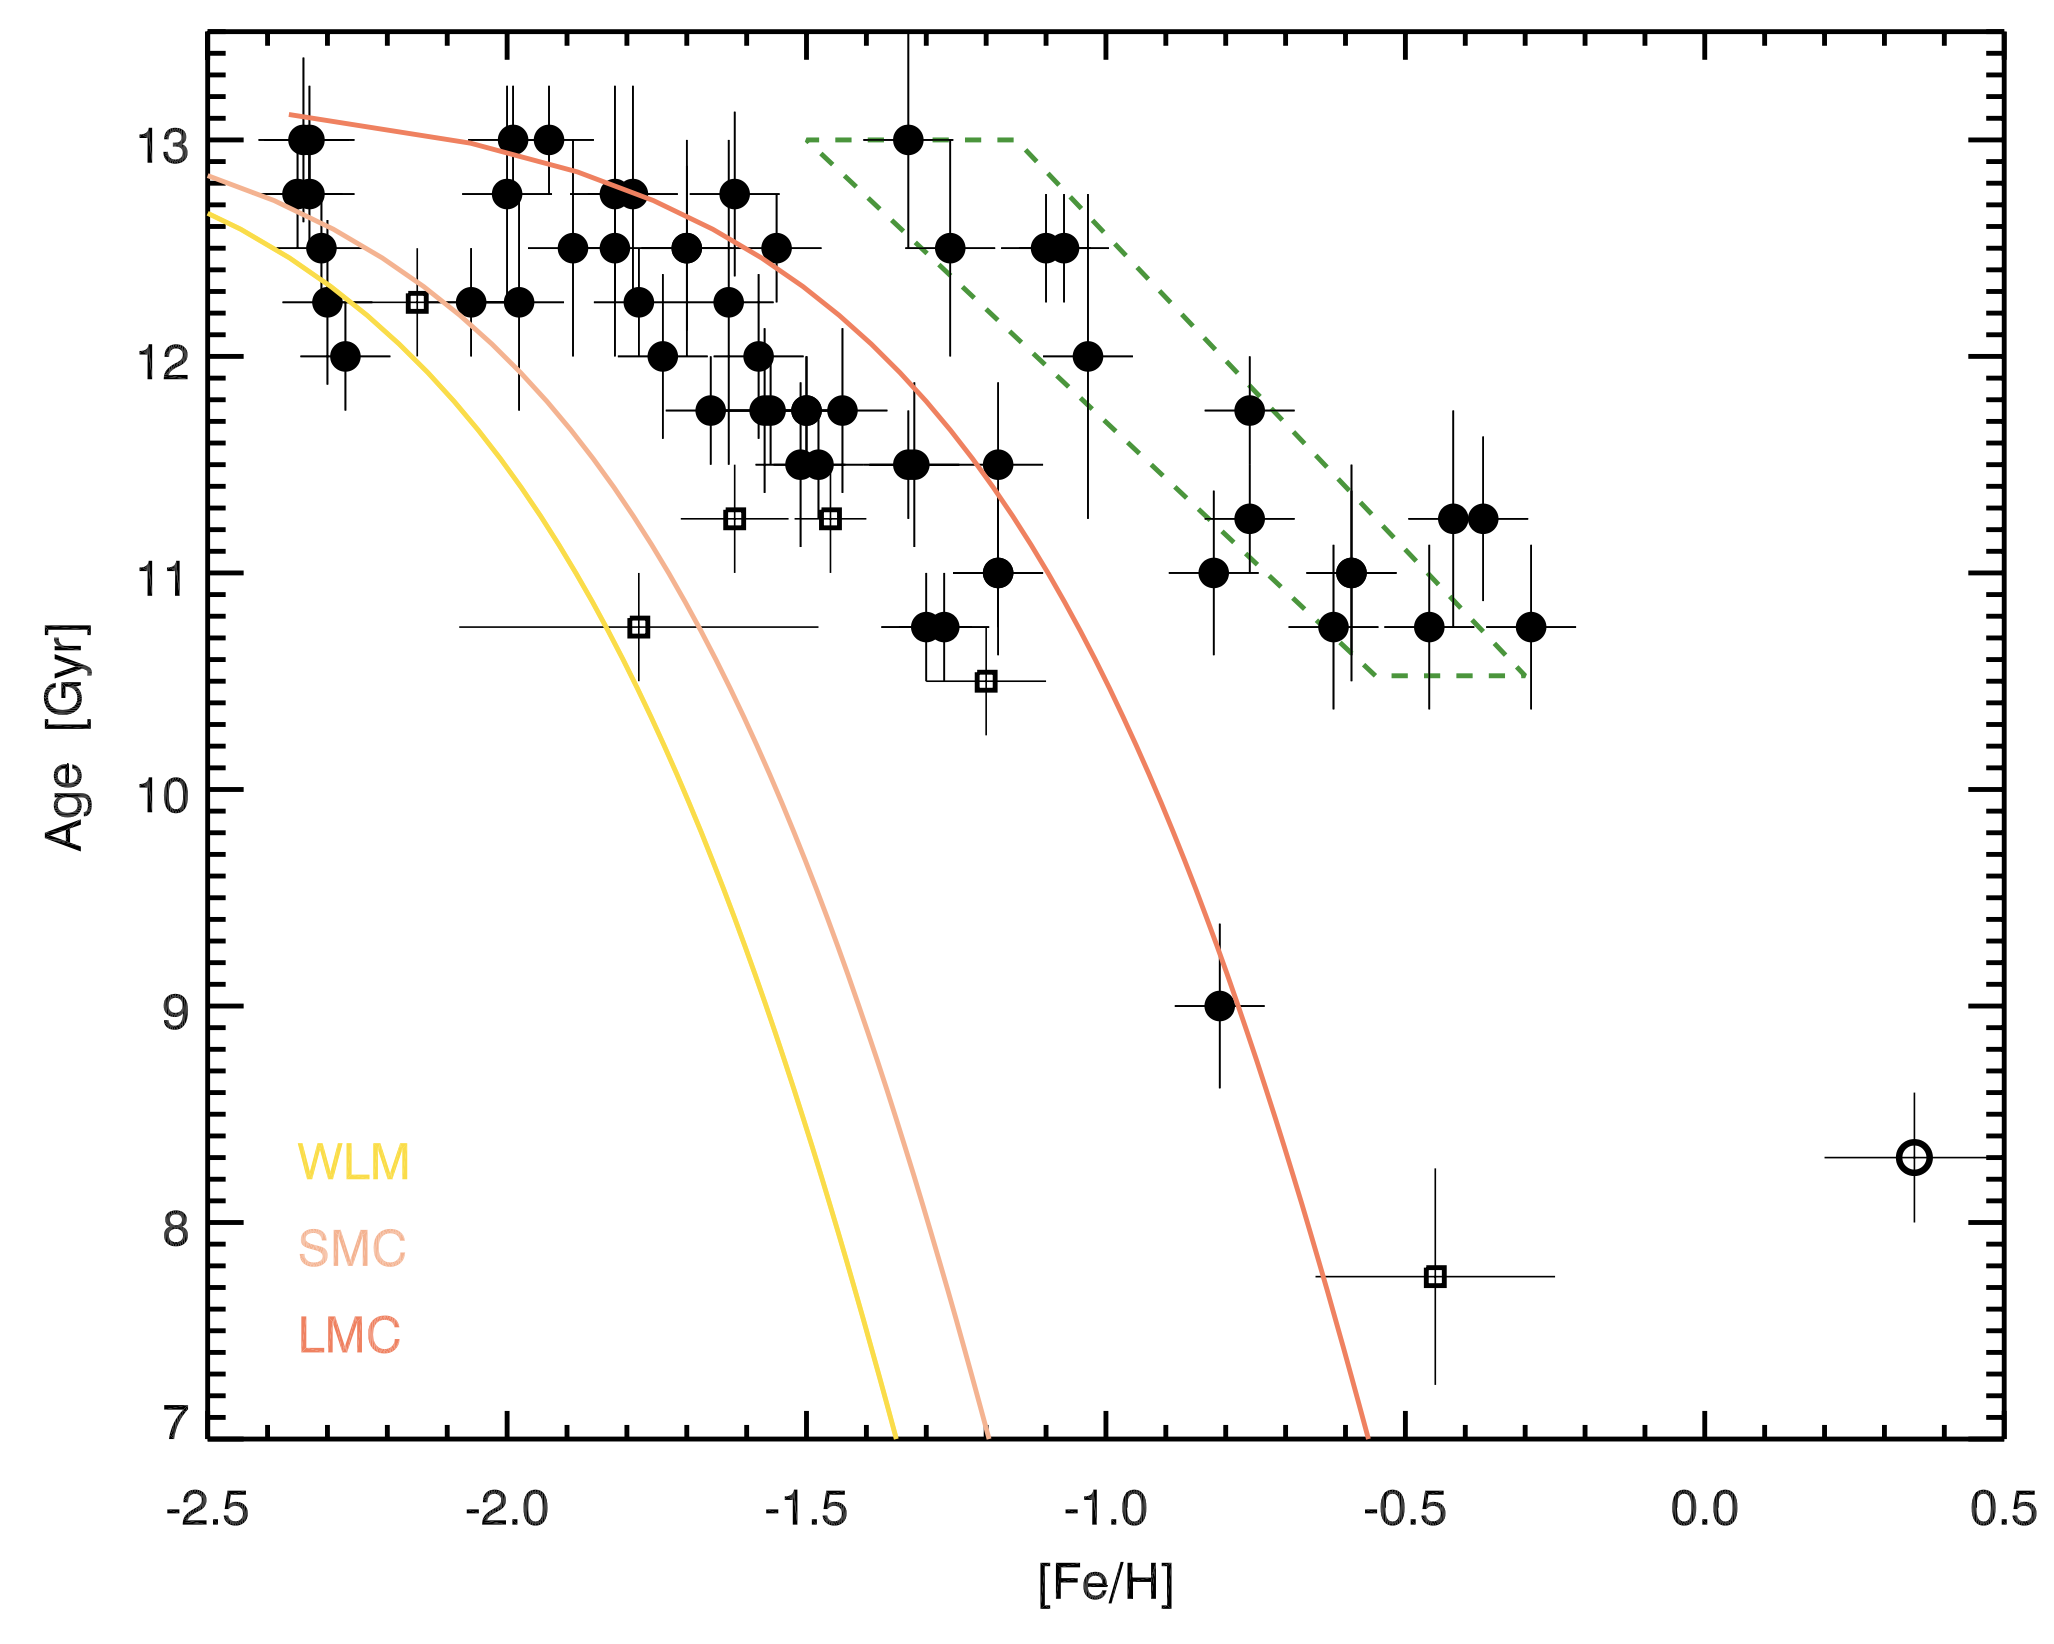
\includegraphics[width=0.65\textwidth]{plots/Intro/Leaman_GCmetal.png}
    
\end{SCfigure}
\\\citet{Leaman...agemetall.MWGCs...2013} use the age-metallicity relation of the \ac{MW} \acp{GC} to distinguish them between in-situ and ex-situ formation and to relate them to their progenitor as shown in Figure \ref{fig:GC_metal_distinguish}. This method can be used in external galaxies to find \acp{GC} accreted from the same satellite.
\\
After the merger, \acp{GC} in the \ac{MW} but also in external galaxies retain a dynamical memory of their progenitor. Their dynamics in the halo depends on the mass and shape of the host. As in Section \ref{subsec:mass_est_MW}, we can use these \acp{GC} as tracers to constrain the gravitational potential.
\\\\
\textbf{Idea}
In this work, we test the idea of adaptive dynamics \citep{Binney...adaptivedynamics...2005} in external galaxies. Adaptive dynamics suggests to use dynamical features (action-angle-frequencies) on similar orbits, be it stellar streams in the halo or resonance moving groups in the disk, and attempts to make these features as sharp as possible in action space. \acp{GC} accreted by one \ac{DG} move on similar orbits. Particles on similar orbits have by definition similar actions. In the wrong potential, the \acp{GC} will not move on similar orbits and the spread in actions will be larger. By minimizing their spread we should be able to constrain the gravitational potential of the galaxy. The big assumption that we test in this work is that even though the exact phase-space distribution of \acp{GC} originating from accreted \acp{DG} depends on the merger parameters such as the infall direction and velocity, and on the disruption process, they might still live on similar orbits. This implies that the \ac{DF} of these accreted objects might be close to a $\delta$-function in action space. If this method works, we will gain more insight in the merger history of the galaxies and on the \ac{DM} and total mass distribution. We test this method in a hydrodynamical cosmological simulation, where we have full 6D phase-space information. To make our investigations comparable to the methods observers use in external galaxies, we fit an analytic axisymmetric potential to the simulation.
\\\\
\textbf{Structure}
This thesis is divided into two major blocks. As a first step we explain in Section \ref{sec:Auriga} how we fit an analytic axisymmetric potential to a hydrodynamical. cosmological simulation. At first thought, this seems to be trivial. But it became obvious that there are many issued to consider. The proposed strategies might help future modellers who want to verify their methods, which require a potential, in simulations. Section \ref{sec:Dynamics} investigates the main idea of this project: testing if it is possible to constrain the gravitational potential of an external galaxy (where we treat simulated galaxies as external galaxies and apply the same techniques observers use) by minimising the spread in action of accreted \acp{GC}. In Section \ref{sec:Discussion} we discuss our results, compare them to current literature, address problems, and give an outlook on how to continue this work. A short summary and conclusion is given in Section \ref{sec:sumconc}.